\section{Quantum Computation}

\begin{comment}
    computational basis states
    bloch spheres
\end{comment}

\subsection{Introduction to Qubits}

In quantum computing, the $\ket 0$ and $\ket 1$ states form the computational basis. They are vectors in a two-dimensional complex Hilbert space $\mathbb{C}^2$.
\begin{equation*}
    \ket 0 = \begin{pmatrix} 1 \\ 0 \end{pmatrix} \qquad\qquad
    \ket 1 = \begin{pmatrix} 0 \\ 1 \end{pmatrix} \qquad
\end{equation*}

We can choose any pair of orthonormal states to form our computational basis. For instance, consider the $\ket +$ and $\ket -$ states.
\begin{equation*}
\begin{gathered}
    \ket + = \frac{1}{\sqrt{2}} (\ket 0 + \ket 1) \qquad\qquad
    \ket - = \frac{1}{\sqrt{2}} (\ket 0 - \ket 1)
\end{gathered}
\end{equation*}

We can depict these computational basis states on a Bloch sphere.
\begin{figure}[H]
\centering
    \begin{minipage}{.4\textwidth}
      \centering
      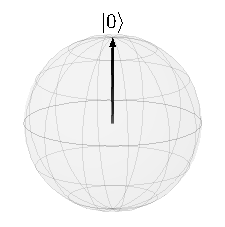
\includegraphics[width=0.5\linewidth]{blochspheres/zero}
      \caption{$\ket 0$ state}
    \end{minipage}%
    \begin{minipage}{.4\textwidth}
      \centering
      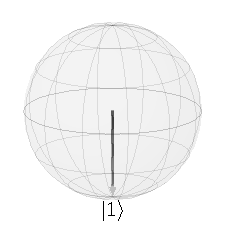
\includegraphics[width=0.5\linewidth]{blochspheres/one}
      \caption{$\ket 1$ state}
    \end{minipage}
    \begin{minipage}{.4\textwidth}
      \centering
      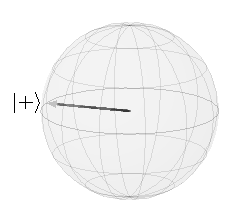
\includegraphics[width=0.5\linewidth]{blochspheres/plus}
      \caption{$\ket +$ state}
    \end{minipage}%
    \begin{minipage}{.4\textwidth}
      \centering
      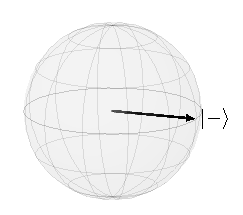
\includegraphics[width=0.5\linewidth]{blochspheres/minus}
      \caption{$\ket -$ state}
    \end{minipage}
\end{figure}

We can choose any pair of orthonormal states to form our computational basis.
\begin{equation*}
\begin{gathered}
    \ket + = \frac{1}{\sqrt{2}} (\ket 0 + \ket 1) \qquad\qquad
    \ket - = \frac{1}{\sqrt{2}} (\ket 0 - \ket 1)
\end{gathered}
\end{equation*}

More generally, any qubit $\ket\psi$ can be represented as complex linear combination of the chosen basis, provided that the qubit state vector is normalised.
\begin{equation*}
\begin{gathered}
    \ket \psi = \alpha\ket 0 + \beta\ket 1 \\
    |\alpha|^2 + |\beta|^2 = 1 \\
    \alpha, \beta \in \mathbb{C}
\end{gathered}
\end{equation*}

